\documentclass{beamer}
%Information to be included in the title page:
\title{Randomized Algorithms for\\Gaussian Process Regression}
\subtitle{GPyTorch Inference Engine}
\author{Matthias Zeller}
%\institute{EPFL}
\date{\today}
\titlegraphic{\includegraphics[height=0.5cm]{report/res/EPFL-logo.pdf}}

\usepackage{biblatex}
\addbibresource{report/references.bib}
%\bibliographystyle{amsalpha}
% make bibliography entries smaller
\renewcommand\bibfont{\scriptsize}

% >>>>>>>>>>>>>>>>>>>>>>>>>>>>>>>>>>>>>> %
%           MATHS                        %
% >>>>>>>>>>>>>>>>>>>>>>>>>>>>>>>>>>>>>> % 
% https://www.overleaf.com/learn/latex/Mathematical_expressions
% https://en.wikibooks.org/wiki/LaTeX/Mathematics
\usepackage{amsmath,amsfonts,amssymb,mathtools, bbold, bbm}

% Algorithms
% https://www.overleaf.com/learn/latex/algorithms
% https://en.wikibooks.org/wiki/LaTeX/Algorithms
%\usepackage[ruled,vlined]{algorithm2e}
%\usepackage{algorithmic}
\usepackage[ruled,vlined]{algorithm2e}
% Colored comments
\newcommand\mycommfont[1]{\ttfamily\textcolor{blue}{#1}}
\SetCommentSty{mycommfont}


% Make mathbb nice (e.g. set of real number R: \mathbb R)
% https://tex.stackexchange.com/questions/58098/what-are-all-the-font-styles-i-can-use-in-math-mode
\AtBeginDocument{
  \DeclareSymbolFont{AMSb}{U}{msb}{m}{n}
  \DeclareSymbolFontAlphabet{\mathbb}{AMSb}
}

% Double struck zero matrix
% https://tex.stackexchange.com/a/399950/217578
\DeclareMathAlphabet{\mymathbb}{U}{BOONDOX-ds}{m}{n}

% Custom commands & operators: vectors, matrice operations, expectations, variance, ...
\newcommand{\vect}[1]{\boldsymbol{\mathbf{#1}}}
\newcommand{\R}{\mathbb R}
\newcommand{\norm}[1]{\Vert #1 \Vert}
\DeclareMathOperator{\trace}{Tr}
\DeclareMathOperator{\E}{\mathbb{E}}
\DeclareMathOperator{\Var}{\mathbb{V}ar}

% Double-bar Identity matrix: with or without size argument
% https://tex.stackexchange.com/questions/409760/detect-no-argument-in-newcommand
\makeatletter
\def\Id{\@ifnextchar[\Id@command{\mathbb I}}
\def\Id@command[#1]{\mathbb I_{#1}}
\makeatother

% Theorem, lemmas, corollaries, proofs, ...
\usepackage{amsthm} % proof
%\newtheorem{theorem}{Theorem}[section]
%\newtheorem{corollary}{Corollary}[theorem]
%\newtheorem{lemma}[theorem]{Lemma}
%\newtheorem{proposition}[theorem]{Proposition}
%\newtheorem*{remark}{Remark}
%\newtheorem{observation}[theorem]{Observation}
% The setup_math.tex file might be included in the slides, where the beamer package already defines theorems & co, so check if they're already defined before adding them
% https://tex.stackexchange.com/questions/41496/how-to-define-an-environment-only-if-it-is-not-defined-yet-using-etoolbox
\ifcsmacro{theorem}{}{
  \let\endtheorem\undefined%
  \newtheorem{theorem}{Theorem}[section]
}
\ifcsmacro{corollary}{}{
  \let\endcorollary\undefined%
  \newtheorem{corollary}{Corollary}[theorem]
}
\ifcsmacro{lemma}{}{
  \let\endlemma\undefined%
  \newtheorem{lemma}[theorem]{Lemma}
}
\ifcsmacro{proposition}{}{
  \let\endproposition\undefined%
  \newtheorem{proposition}[theorem]{Proposition}
}
\ifcsmacro{remark}{}{
  \let\endremark\undefined%
  \newtheorem*{remark}{Remark}
}
\ifcsmacro{observation}{}{
  \let\endobservation\undefined%
  \newtheorem{observation}[theorem]{Observation}
}


% <<<<<<<<<<<<<<<<<<<<<<<<<<<<<<<<<<<<<< %
%           MATHS                        %
% <<<<<<<<<<<<<<<<<<<<<<<<<<<<<<<<<<<<<< %

\AtBeginSection[]{
  \begin{frame}
  \vfill
  \centering
  \begin{beamercolorbox}[sep=8pt,center,shadow=true,rounded=true]{title}
    \usebeamerfont{title}\insertsectionhead\par%
  \end{beamercolorbox}
  \vfill
  \end{frame}
}

\usepackage{comment}
\usepackage{multirow}
\usepackage{tikz}
\usetikzlibrary{matrix}
\usetikzlibrary{shadows}
\tikzset{c/.style={fill=yellow}}
\tikzset{mystyle/.style={matrix of nodes,
        nodes in empty cells,
        row sep=-\pgflinewidth,
        column sep=-\pgflinewidth,
        nodes={draw,minimum width=1cm,minimum height=1cm,anchor=center}}}

\begin{document}

\frame{\titlepage}

\begin{frame}{Introduction to Gaussian Process Regression}
\begin{itemize}[<+->]
    \item Task: approximate an unknown function $f$ given its noisy evaluations:
    \begin{equation*}
        y_i = f(\vect x_i) + \epsilon_i, \quad \epsilon_i \stackrel{\text{iid}}{\sim} \mathcal N(0, \sigma^2)
    \end{equation*}
    \item Gaussian Process (GP) regression: Bayesian method
    \item Model $f$ as a stochastic process with a GP prior
    \begin{equation*}
        f \sim \mathcal{GP}(\mu(\vect x), k(\vect x, \vect x'))
    \end{equation*}
    \item We will call $k$ the kernel function
    \item Notation: collect $\vect y = (y_1, \ldots, y_n)$, $X = \begin{bmatrix}
    \vect x_1 & \dots & \vect x_n
    \end{bmatrix}$
    \item The observations have a Gaussian prior
    \begin{equation*}
        \vect y \mid X \sim \mathcal N(\vect 0, \widehat K_{XX})
    \end{equation*}
    \item SPD Kernel matrix: $(K_{XX})_{ij} = k(\vect x_i, \vect x_j)$, $\widehat K_{XX} = K_{XX} + \sigma^2 \Id$
\end{itemize}
\end{frame}

\begin{frame}{Introduction to Gaussian Process Regression}
\begin{itemize}[<+->]
    \item Model $f$ as a stochastic process with a GP prior
    \begin{equation*}
        f \sim \mathcal{GP}(\mu(\vect x), k(\vect x, \vect x'))
    \end{equation*}
    \item The observations have a Gaussian prior
    \begin{equation*}
        \vect y \mid X \sim \mathcal N(\vect 0, \widehat K_{XX})
    \end{equation*}
    \item Use the model: evaluate $f$ at a test point $\vect x^\star$ by conditioning on training observations $\vect y$
    \item Posterior distribution: 
    \begin{equation*}
        f(\vect x^\star) \mid \vect y, X, \vect x^\star \sim \mathcal N
    \end{equation*}
    \item Takeaway: the most important quantity are the kernel function and the kernel matrix:
    \begin{equation*}
        (K_{XX})_{ij} = k(\vect x_i, \vect x_j), \quad \widehat K_{XX} = K_{XX} + \sigma^2 \Id
    \end{equation*}
\end{itemize}
\end{frame}

\begin{comment}
\begin{frame}{Introduction}
\begin{itemize}[<+->]
    \item Given noisy observations of some unknown function $f$,
        \begin{equation*}
        y_i = f(\vect x_i) + \epsilon_i, \quad \epsilon_i \stackrel{\text{iid}}{\sim} \mathcal N(0, \sigma^2)
    \end{equation*}
    \item We wish to approximate $f$ 
    
    %\item Gaussian Process Regression: extension of Bayesian linear regression
    \item Model the prior $f \sim \mathcal{GP}(\mu(\vect x), k(\vect x, \vect x'))$
    \item $k(\vect x, \vect x')$ is the covariance, or \emph{kernel} function
    \item Important quantity: SPD kernel matrix 
    \begin{equation*}
        (\widehat K_{XX})_{ij} = k(\vect x_i, \vect x_j) + \delta_{ij}\sigma^2
    \end{equation*}
\end{itemize}
\end{frame}

\begin{frame}{Introduction}
\begin{itemize}[<+->]
    
    \item Given some data $X = (\vect x_1, \ldots, \vect x_n) \in \R^{d \times n}$ and $\vect y \in \R^n$, assume there is an unknown function $f: \R^d \to \R$:
    \begin{equation*}
        y_i = f(\vect x_i) + \epsilon_i, \quad \epsilon_i \stackrel{\text{iid}}{\sim} \mathcal N(0, \sigma^2)
    \end{equation*}
    
    \item Gaussian Process Regression: model unknown function as a Gaussian Process with prior $f \sim \mathcal{GP}(\mu, k)$
    \item $k$ is the covariance, or \emph{kernel} function (we set $\mu = 0$)
    \item Prior function values at $\vect x_i$ are jointly Gaussian,
    \begin{equation*}
        \vect y \mid X \sim \mathcal N(\vect 0, \widehat K_{XX})
    \end{equation*}
    \item Kernel matrix $(\widehat K_{XX})_{ij} = k(\vect x_i, \vect x_j) + \delta_{ij} \sigma^2$
    \item The predictive mean at a new point $\vect x^\star$ is the conditional mean:
    \begin{equation*}
        \E_{f(\vect x^\star) \sim \mathcal{GP}(0, k)}[f \mid \vect y,  X, \vect x^\star ] = \vect k_{X \vect x^\star}^\top \widehat K_{XX}^{-1} \vect y
    \end{equation*}
\end{itemize}

\end{frame}
\end{comment}


\begin{frame}{Kernel functions}
\begin{itemize}[<+->]
    \item Crucial step: choice of the kernel $k$
    \item This encodes prior knowledge on our function $f$
    \item e.g., controls the smoothness of $f$
    \item Examples of most popular kernels:
    \begin{itemize}
        \item Squared exponential $k_\text{SE}(\vect x_i, \vect x_j ; \; \ell)$
        \item Matern kernel $k_\text{Matern}(\vect x_i, \vect x_j ; \; \ell, \nu)$
        \item $\ell, \nu$ are additional parameters
    \end{itemize}
    \item Example of priors drawn from $f \sim \mathcal{GP}(0, k)$:
\end{itemize}
\pause\begin{figure}
    \centering
    \includegraphics[clip, trim=11cm 0cm 0cm 0cm, width=0.75\textwidth]{res/covariance_overview.pdf}
    \label{fig:my_label}
\end{figure}
\end{frame}

\begin{frame}{Training a Gaussian Process}
\begin{itemize}[<+->]
    \item Unknown parameters $\vect\theta$: noise variance $\sigma^2$, kernel parameters (e.g. lengthscale $\ell$)
    \item Estimate $\vect\theta$ from the data with maximum likelihood estimation
    \item Gradient descent: need to evaluate the likelihood $\mathcal L(\vect\theta \mid X, \vect y)$ and its gradient $\nabla_{\vect\theta} \mathcal L(\vect\theta \mid X, \vect y) $
    \pause
    {\small \begin{align*}
        \mathcal L(\vect\theta \mid X, \vect y) 
    :=& \log p(\vect y \mid X, \vect \theta) \nonumber\\
    =& - \frac 1 2 \vect y^\top \widehat K_{XX}^{-1} \vect y - \frac 1 2 \log \det \left( \widehat K_{XX} \right) - \frac n 2 \log(2\pi) \label{eq:marginal_log_likelihood}\\[0.5cm]
    \frac{d \mathcal L}{d \theta_i} (\vect \theta \mid X, \vect y) 
    =& \, \frac 1 2 \vect y^\top \widehat K_{XX}^{-1} \frac{d \widehat K_{XX}}{d\theta_i} \widehat K_{XX}^{-1} \vect y - \frac 1 2 \trace \left( \widehat K_{XX}^{-1} \frac{d \widehat K_{XX}}{d\theta_i} \right)
    \end{align*}}
\end{itemize}
\end{frame}

\begin{frame}{Training a Gaussian Process}
\begin{itemize}[<+->]
    \item Computation of $\mathcal L(\vect\theta \mid X, \vect y)$,  $\nabla_{\vect\theta} \mathcal L(\vect\theta \mid X, \vect y) $ dominated by 
    \begin{itemize}
        \item Linear solve $\widehat K_{XX}^{-1} \vect y$
        \item Log determinant $\log \det \left( \widehat K_{XX} \right)$
        \item Trace term $\trace \left( \widehat K_{XX}^{-1} \frac{d \widehat K_{XX}}{d\theta_i} \right)$
    \end{itemize}
    \item Some inference engines use the Cholesky decomposition $\widehat K_{XX} = L L^\top$
    \item Cubic-time complexity $\mathcal O(n^3)$ with $n$ the number of observations
    \item Cholesky does not scale to large datasets
    \item Alternative: iterative methods 
\end{itemize}
\end{frame}

\begin{frame}{GPyTorch}
\begin{itemize}[<+->]
    \item GPyTorch \cite{gardner_gpytorch_2021}: Gaussian Process Regression library build on top of PyTorch
    %\item Strength: the user only provides blackbox matrix-matrix multiplication oracles $A \mapsto \widehat K_{XX} A$, $A \mapsto \frac{d \widehat K_{XX}}{d\theta} A$
    \item Core of GPyTorch: modified batched conjugate gradients (mBCG) algorithm
    \item mBCG approximates the solution of 
    \begin{equation*}
    \widehat K_{XX} \begin{bmatrix} \vect u_0 & \vect u_1 & \dots & \vect u_N \end{bmatrix} = 
    \begin{bmatrix} \vect y & \vect z_1 & \dots & \vect z_N \end{bmatrix} \; ,
    \quad \vect z_i \sim \mathcal N(\vect 0, \Id)
    \end{equation*}
    \item Additionally, return partial Lanczos tridiagonalizations $\tilde T_1, \ldots, \tilde T_N$ of $\widehat K_{XX}$ with starting vectors $\vect z_i$
    \item $\tilde T_i$ can be obtained from conjugate gradients
\end{itemize}
\end{frame}

\begin{frame}{mBCG to compute {\normalsize $\widehat K_{XX}^{-1} \vect y$},  \textcolor{gray}{\normalsize{$\trace \left(\widehat K_{XX}^{-1} \frac{d \widehat K_{XX}}{d\theta} \right)$, $\log\det( \widehat K_{XX} )$}}}
\begin{itemize}[<+->]
    \item mBCG returns
    \begin{equation*}
        \tilde T_1, \ldots, \tilde T_N \text{ and } \begin{bmatrix} \tilde{\vect u}_0 & \tilde{\vect u}_1 & \dots & \tilde{\vect u}_N \end{bmatrix} \approx 
    \widehat K_{XX}^{-1} \begin{bmatrix} \vect y & \vect z_1 & \dots & \vect z_N \end{bmatrix}
    \end{equation*}
    \item Readily get the linear solve from the output $\tilde{\vect u}_0$
\end{itemize}
\end{frame}

\begin{frame}{mBCG to compute \textcolor{gray}{\normalsize $\widehat K_{XX}^{-1} \vect y$},  \normalsize{$\trace \left(\widehat K_{XX}^{-1} \frac{d \widehat K_{XX}}{d\theta} \right)$}, \textcolor{gray}{\normalsize $\log\det( \widehat K_{XX} )$}}
\begin{itemize}[<+->]
    \item mBCG returns
    \begin{equation*}
        \tilde T_1, \ldots, \tilde T_N \text{ and } \begin{bmatrix} \tilde{\vect u}_0 & \tilde{\vect u}_1 & \dots & \tilde{\vect u}_N \end{bmatrix} \approx 
    \widehat K_{XX}^{-1} \begin{bmatrix} \vect y & \vect z_1 & \dots & \vect z_N \end{bmatrix}
    \end{equation*}
    \item Stochastic trace approximation for the trace term:
    \begin{align*}
        \uncover<+->{\trace \left(\widehat K_{XX}^{-1} \frac{d \widehat K_{XX}}{d\theta} \right)
        &= \E_{\mathcal N(\vect 0, \Id)} \left[ \vect z^\top \widehat K_{XX}^{-1}  \frac{d \widehat K_{XX}}{d\theta} \vect z \right]}\\
        \uncover<+->{&\approx \frac{1}{N} \sum_{i=1}^N \left( \vect z_i^\top \widehat K_{XX}^{-1} \right) \left( \frac{d \widehat K_{XX}}{d\theta} \vect z_i \right)} \\
        \uncover<+->{&\approx \frac{1}{N} \sum_{i=1}^N \tilde{\vect u}_i^\top \frac{d \widehat K_{XX}}{d\theta} \vect z_i}
    \end{align*}
\end{itemize}
\end{frame}


\begin{frame}{mBCG to compute \textcolor{gray}{\normalsize $\widehat K_{XX}^{-1} \vect y$,  \normalsize{$\trace \left(\widehat K_{XX}^{-1} \frac{d \widehat K_{XX}}{d\theta} \right)$}}, {\normalsize $\log\det( \widehat K_{XX} )$}}
\begin{itemize}[<+->]
    \item mBCG returns
    \begin{equation*}
        \tilde T_1, \ldots, \tilde T_N \text{ and } \begin{bmatrix} \tilde{\vect u}_0 & \tilde{\vect u}_1 & \dots & \tilde{\vect u}_N \end{bmatrix} \approx 
    \widehat K_{XX}^{-1} \begin{bmatrix} \vect y & \vect z_1 & \dots & \vect z_N \end{bmatrix}
    \end{equation*}
    \item For $\widehat K_{XX}$ SPD,
    \begin{align*}
        \uncover<+->{\log\det \widehat K_{XX} &= \trace \log \widehat K_{XX}\\}
        \uncover<+->{&= \E[\vect z^\top \log(\widehat K_{XX}) \vect z]}
    \end{align*}
    \item The matrix log is too expensive to compute
    \item Lanczos quadrature to approximate $\vect z^\top \log(\widehat K_{XX}) \vect z$
    \item Final estimate: stochastic Lanczos quadrature
    %\item Approximate the trace log with stochastic Lanczos quadrature: after $n$ Lanczos steps, $T = Q^\top \widehat K_{XX} Q$
    \begin{align*}
        \frac{1}{N} \sum_{i=1}^N \norm{\vect z_i}_2^2 \, \vect e_1^\top \log ( \tilde T_i ) \, \vect e_1
        \approx \log \det \widehat K_{XX} 
        %&= \E_{\mathcal N(\vect 0, \Id)} \left[ \norm{\vect z}_2^2 \, \vect e_1^\top (\log T) \vect e_1 \right]\\&\approx 
    \end{align*}
\end{itemize}
\end{frame}

\begin{frame}{Need for preconditioning}
\begin{itemize}[<+->]
    \item Recall mBCG is essentially CG + Lanczos
    \item Notation: $\kappa \equiv \kappa(\widehat K_{XX})$
    \item CG convergence depends on $(\sqrt{\kappa} - 1) / (\sqrt{\kappa} + 1)$
    \item Lanczos for logdet estimation: we roughly need the number of steps $\propto \sqrt{\kappa}$ (\cite{ubaru_fast_2017}, \cite{cortinovis_randomized_2021})
\end{itemize}
\end{frame}


\begin{frame}{Preconditioning mBCG}
\begin{itemize}[<+->]
    \item Assume we have an SPD preconditioner $P$
    \item Precondition the system $\widehat K_{XX} \vect u = \vect z$ as:
    \begin{equation*}
        \left( P^{-\frac 1 2} \widehat K_{XX} P^{-\frac 1 2} \right) \left( P^{\frac 1 2} \vect u\right) = P^{-\frac 1 2} \vect z
    \end{equation*}
    \item We now compute tridiagonalizations of the preconditioned matrix, i.e. we compute the log-det of the preconditioned matrix
    \item Recover the original log-det:
    \begin{equation*}
        \log\det \widehat K_{XX} = 
        \underbrace{ 
            \vphantom{\left(P^{-\frac 1 2}  \right)} 
            \log \det P
        }_{\text{exact}} 
        + \underbrace{ 
            \log \det \left(P^{-\frac 1 2} \widehat K_{XX} P^{-\frac 1 2} \right)
        }_{\text{random estimation}}
    \end{equation*}
    \item Which preconditioner $P$ to use ?
    %\item Unbiasedness of the trace estimator: $P^{-1/2} \vect z \sim \mathcal N(\vect 0, \Id)$, i.e. $\vect z \sim \mathcal N(\vect 0, P)$
\end{itemize}
\end{frame}

\begin{frame}{Preconditioning mBCG with Partial Pivoted Cholesky}
\begin{itemize}
    \item<1-> GPyTorch uses pivoted Cholesky (Cholesky with permutation)
    \item<2-> The (full) algorithm computes the decomposition $ L  L^\top = K_{XX}$
    \item<3-> $ L$ is lower triangular up to some row permutations
\end{itemize}

\onslide<3->\begin{table}
\centering
\renewcommand{\arraystretch}{1.5}
\begin{tabular}{cccc}
\multirow{3}{*}{\resizebox{2cm}{!}{
\begin{tikzpicture}
	\draw[fill = black] (0.0, 5.0) rectangle (1.0, 6.0);
	\draw[fill = black] (1.0, 5.0) rectangle (2.0, 6.0);
	\draw[fill = black] (2.0, 5.0) rectangle (3.0, 6.0);
	\draw[fill = black] (3.0, 5.0) rectangle (4.0, 6.0);
	\draw[fill = black] (4.0, 5.0) rectangle (5.0, 6.0);
	\draw[fill = white] (5.0, 5.0) rectangle (6.0, 6.0);
	\draw[fill = black] (0.0, 4.0) rectangle (1.0, 5.0);
	\draw[fill = black] (1.0, 4.0) rectangle (2.0, 5.0);
	\draw[fill = black] (2.0, 4.0) rectangle (3.0, 5.0);
	\draw[fill = black] (3.0, 4.0) rectangle (4.0, 5.0);
	\draw[fill = black] (4.0, 4.0) rectangle (5.0, 5.0);
	\draw[fill = black] (5.0, 4.0) rectangle (6.0, 5.0);
	\draw[fill = black] (0.0, 3.0) rectangle (1.0, 4.0);
	\draw[fill = black] (1.0, 3.0) rectangle (2.0, 4.0);
	\draw[fill = black] (2.0, 3.0) rectangle (3.0, 4.0);
	\draw[fill = white] (3.0, 3.0) rectangle (4.0, 4.0);
	\draw[fill = white] (4.0, 3.0) rectangle (5.0, 4.0);
	\draw[fill = white] (5.0, 3.0) rectangle (6.0, 4.0);
	\draw[fill = black] (0.0, 2.0) rectangle (1.0, 3.0);
	\draw[fill = black] (1.0, 2.0) rectangle (2.0, 3.0);
	\draw[fill = black] (2.0, 2.0) rectangle (3.0, 3.0);
	\draw[fill = black] (3.0, 2.0) rectangle (4.0, 3.0);
	\draw[fill = white] (4.0, 2.0) rectangle (5.0, 3.0);
	\draw[fill = white] (5.0, 2.0) rectangle (6.0, 3.0);
	\draw[fill = black] (0.0, 1.0) rectangle (1.0, 2.0);
	\draw[fill = white] (1.0, 1.0) rectangle (2.0, 2.0);
	\draw[fill = white] (2.0, 1.0) rectangle (3.0, 2.0);
	\draw[fill = white] (3.0, 1.0) rectangle (4.0, 2.0);
	\draw[fill = white] (4.0, 1.0) rectangle (5.0, 2.0);
	\draw[fill = white] (5.0, 1.0) rectangle (6.0, 2.0);
	\draw[fill = black] (0.0, 0.0) rectangle (1.0, 1.0);
	\draw[fill = black] (1.0, 0.0) rectangle (2.0, 1.0);
	\draw[fill = white] (2.0, 0.0) rectangle (3.0, 1.0);
	\draw[fill = white] (3.0, 0.0) rectangle (4.0, 1.0);
	\draw[fill = white] (4.0, 0.0) rectangle (5.0, 1.0);
	\draw[fill = white] (5.0, 0.0) rectangle (6.0, 1.0);
\end{tikzpicture}}} & &
\multirow{3}{*}{\resizebox{2cm}{!}{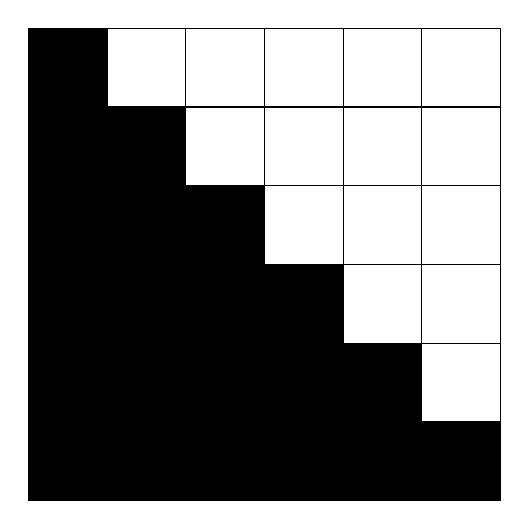
\begin{tikzpicture}
	\draw[fill = black] (0.0, 5.0) rectangle (1.0, 6.0);
	\draw[fill = white] (1.0, 5.0) rectangle (2.0, 6.0);
	\draw[fill = white] (2.0, 5.0) rectangle (3.0, 6.0);
	\draw[fill = white] (3.0, 5.0) rectangle (4.0, 6.0);
	\draw[fill = white] (4.0, 5.0) rectangle (5.0, 6.0);
	\draw[fill = white] (5.0, 5.0) rectangle (6.0, 6.0);
	\draw[fill = black] (0.0, 4.0) rectangle (1.0, 5.0);
	\draw[fill = black] (1.0, 4.0) rectangle (2.0, 5.0);
	\draw[fill = white] (2.0, 4.0) rectangle (3.0, 5.0);
	\draw[fill = white] (3.0, 4.0) rectangle (4.0, 5.0);
	\draw[fill = white] (4.0, 4.0) rectangle (5.0, 5.0);
	\draw[fill = white] (5.0, 4.0) rectangle (6.0, 5.0);
	\draw[fill = black] (0.0, 3.0) rectangle (1.0, 4.0);
	\draw[fill = black] (1.0, 3.0) rectangle (2.0, 4.0);
	\draw[fill = black] (2.0, 3.0) rectangle (3.0, 4.0);
	\draw[fill = white] (3.0, 3.0) rectangle (4.0, 4.0);
	\draw[fill = white] (4.0, 3.0) rectangle (5.0, 4.0);
	\draw[fill = white] (5.0, 3.0) rectangle (6.0, 4.0);
	\draw[fill = black] (0.0, 2.0) rectangle (1.0, 3.0);
	\draw[fill = black] (1.0, 2.0) rectangle (2.0, 3.0);
	\draw[fill = black] (2.0, 2.0) rectangle (3.0, 3.0);
	\draw[fill = black] (3.0, 2.0) rectangle (4.0, 3.0);
	\draw[fill = white] (4.0, 2.0) rectangle (5.0, 3.0);
	\draw[fill = white] (5.0, 2.0) rectangle (6.0, 3.0);
	\draw[fill = black] (0.0, 1.0) rectangle (1.0, 2.0);
	\draw[fill = black] (1.0, 1.0) rectangle (2.0, 2.0);
	\draw[fill = black] (2.0, 1.0) rectangle (3.0, 2.0);
	\draw[fill = black] (3.0, 1.0) rectangle (4.0, 2.0);
	\draw[fill = black] (4.0, 1.0) rectangle (5.0, 2.0);
	\draw[fill = white] (5.0, 1.0) rectangle (6.0, 2.0);
	\draw[fill = black] (0.0, 0.0) rectangle (1.0, 1.0);
	\draw[fill = black] (1.0, 0.0) rectangle (2.0, 1.0);
	\draw[fill = black] (2.0, 0.0) rectangle (3.0, 1.0);
	\draw[fill = black] (3.0, 0.0) rectangle (4.0, 1.0);
	\draw[fill = black] (4.0, 0.0) rectangle (5.0, 1.0);
	\draw[fill = black] (5.0, 0.0) rectangle (6.0, 1.0);
\end{tikzpicture}}}
\\
& $\longleftrightarrow$ &
\\
\end{tabular}
\end{table}

\vspace{0.8cm}

\begin{itemize}
    \item<4-> After $k < n$ steps, we obtain a rank $k$ approximation $L_k L_k^\top \approx K_{XX}$
    \item<5-> The SPD preconditioner is $\widehat P_k = L_k L_k^\top + \sigma^2 \Id \approx \widehat K_{XX}$
\end{itemize}

\end{frame}



\begin{frame}{Preconditioning Kernel Matrices with Pivoted Cholesky}
\begin{itemize}[<+->]
    \item The SPD preconditioner is $\widehat P_k = L_k L_k^\top + \sigma^2 \Id \approx \widehat K_{XX}$
    \item Pivoted Cholesky is costly, aim for small rank $k$
    \item We want to bound the condition number $\kappa ( \widehat P_k^{-\frac 1 2} \widehat K_{XX} \widehat P_k^{-\frac 1 2} )$ in function of $k$
    \item One can show (\cite{gardner_gpytorch_2021}, \cite{harbrecht_low-rank_2012})
    \begin{equation*}
        \kappa \left( \widehat P_k^{-\frac 1 2} \widehat K_{XX} \widehat P_k^{-\frac 1 2}  \right) \le (1 + \mathcal O(n\Gamma_k \lambda_k))^2
    \end{equation*}
    \item $\lambda_k$: $k$th largest eigenvalue of $\widehat K_{XX}$
    \item $\Gamma_k$: some growing factor arising from pivoted Cholesky, depends on $\widehat K_{XX}$
    \item Any guarantee that $\Gamma_k \lambda_k \to 0$ ?
\end{itemize}
\end{frame}


\begin{frame}{Preconditioning Kernel Matrices with Pivoted Cholesky}
\begin{itemize}[<+->]
    \item One can show (\cite{gardner_gpytorch_2021}, \cite{harbrecht_low-rank_2012})
    \begin{equation*}
        \kappa \left( \widehat P_k^{-\frac 1 2} \widehat K_{XX} \widehat P_k^{-\frac 1 2}  \right) \le (1 + \mathcal O(n\Gamma_k \lambda_k))^2
    \end{equation*}
    \item No expression for $\Gamma_k$, but $\Gamma_k = \mathcal O(4^k)$
    \item One can characterize the decay of $\lambda_k$ (\cite{gardner_gpytorch_2021, banerjee_parallel_2013, rasmussen_gaussian_2005}):
    \vspace{0.5cm}
    \resizebox{\textwidth}{!}{%
    \begin{tabular}{l|ll|ll}
    \hline
    {} & \multicolumn{2}{l}{Uniform data} & \multicolumn{2}{l}{Gaussian Data} \\
    {} & SE & Matern & SE & Matern \\
    \hline
    Dimension 1  &       $o(e^{-bk})$ &           $\mathcal O(k^{-b})$ &       $\mathcal O(e^{-bk})$ &           ? \\
    Dimension $>$ 1 &       $\mathcal O(e^{-bk^{1/d}})$ &           ? &       ? &           ? \\
    \hline
    \end{tabular}%
    }
    \item 1D uniform data with SE kernel: only case for which we know $\Gamma_k \lambda_k \to 0$
\end{itemize}
\end{frame}


\begin{comment}

\begin{frame}{Preconditioning Kernel Matrices with Pivoted Cholesky}
\begin{itemize}[<+->]
    \item Let $E_k := K_{XX} - L_kL_k^\top$ be the low-rank approximation error of pivoted Cholesky
    \item 
    \item Bound the condition number: for some constant $c$,
    \begin{equation*}
        \kappa \left( \widehat P_k^{-\frac 1 2} \widehat K_{XX} \widehat P_k^{-\frac 1 2} \right) \le (1 + c \trace(E_k) )^2
    \end{equation*}
    \item Bound the trace: for some growing factor $\Gamma_k$, with $\lambda_k$ the $k$ largest eigenvalue,
    \begin{equation*}
        \trace(E_k) \le n \Gamma_k \lambda_k(K_{XX}) \;,
    \end{equation*}
    \item If $\lambda_k = \mathcal O(1/\Gamma_k)$, then
    \begin{equation*}
        \kappa \left( \widehat P_k^{-\frac 1 2} \widehat K_{XX} \widehat P_k^{-\frac 1 2} \right) \le 1 + \mathcal O(n \Gamma_k \lambda_k)
    \end{equation*}
\end{itemize}
\end{frame}

\begin{frame}{Preconditioning Kernel Matrices with Pivoted Cholesky}
\begin{proposition}
Let $L_kL_k^\top$ be the rank $k$ pivoted Cholesky approximation of $K_{XX}$, then the condition number of the preconditioned matrix satisfies
{\small
\begin{equation*}
    \kappa \left( \widehat P_k^{-\frac 1 2} \widehat K_{XX} \widehat P_k^{-\frac 1 2} \right) \le (1 + c \trace(E_k) )^2
\end{equation*}}
with $E_k = K_{XX} - L_kL_k^\top$ the error matrix and $c$ some constant.
\end{proposition}
\pause
\begin{theorem}
With $L_k$ the $k$-step pivoted Cholesky factor of $K_{XX}$, then the trace of the low-rank approximation error satisfies

\begin{equation*}
    \trace(E_k) \le n \Gamma_k \lambda_k(K_{XX}) \;,
\end{equation*}

for some growing factor $\Gamma_k$ that depends on $K_{XX}$. In the worst case, $\Gamma_k = \mathcal O(4^k)$. 

\end{theorem}
\end{frame}

\begin{frame}{Preconditioning Kernel Matrices with Pivoted Cholesky}
\begin{corollary}
If the spectrum of the kernel matrix decays faster than $1/\Gamma_k$, then

\begin{equation*}
    \kappa \left( \widehat P_k^{-\frac 1 2} \widehat K_{XX} \widehat P_k^{-\frac 1 2} \right) = 1 + \mathcal O(n \Gamma_k \lambda_k) \;,
\end{equation*}

and mBCG converges as 
\begin{equation*}
    \norm{\vect u^\star - \vect u_m}_{\widehat K_{XX}} \le 2 \left(\frac{1}{1 + \mathcal O((n\Gamma_k\lambda_k)^{-1/2})}\right)^m \norm{\vect u^\star - \vect u_0}_{\widehat K_{XX}}
\end{equation*}

\end{corollary}
\end{frame}
\end{comment}

\begin{comment}

\begin{frame}{Recap}
\begin{itemize}[<+->]
    \item Compute $\widehat K_{XX}^{-1} \vect y$ with CG, $\log \det \left( \widehat K_{XX} \right)$ with stochastic Lanczos quadrature, $\trace \left( \widehat K_{XX}^{-1} \frac{d \widehat K_{XX}}{d\theta_i} \right)$ with stochastic trace estimation + CG
    \item The need for preconditioning and its efficiency depends on the spectral decay of the kernel matrix 
    \item We have
    \begin{equation*}
        \kappa ( \widehat P_k^{-\frac 1 2} \widehat K_{XX} \widehat P_k^{-\frac 1 2} ) \le (1 + c \trace(E_k))^2 \le ( 1 + c n \Gamma_k \lambda_k(K_{XX}))^2
    \end{equation*}
    \item Upper bounds on $\lambda_k(K_{XX})$ is proportional to:
\end{itemize}
\onslide<4>\begin{center}
    \begin{tabular}{l|ll|ll}
    \hline
    {} & \multicolumn{2}{l}{Compact $D$} & \multicolumn{2}{l}{Non-compact $D$} \\
    {} & SE & Matern & SE & Matern \\
    \hline
    Univariate   &       $e^{-bk}$ &           $k^{-2\lceil \nu \rceil}$ {\tiny (uniform data)} &       $e^{-bk}$ &           ? \\
    Multivariate &       $e^{-bk^{1/d}}$ &           ? &       ? &           ? \\
    \hline
    \end{tabular}
\end{center}
\end{frame}
\end{comment}


\section{Numerical Experiments}

\begin{comment}
\begin{frame}{Effect of Data Distribution on Spectral Decay}
\begin{itemize}
    \item Sample data $\vect x_1, \ldots, \vect x_{100} \sim \mathcal D$
    \item Compute $\lambda_i(K_{XX})$ and average over 10 runs
\end{itemize}
\begin{figure}
    \centering
    \begin{overprint}
    \onslide<1>\includegraphics[width=\textwidth]{res/kernel_eigenvalues_dimension_empty_4.pdf}
    \onslide<2>\includegraphics[width=\textwidth]{res/kernel_eigenvalues_dimension_empty_3.pdf}
    \onslide<3>\includegraphics[width=\textwidth]{res/kernel_eigenvalues_dimension_empty_2.pdf}
    \onslide<4>\includegraphics[width=\textwidth]{res/kernel_eigenvalues_dimension_empty_1.pdf}
    \onslide<5>\includegraphics[width=\textwidth]{res/kernel_eigenvalues_dimension.pdf}
    \end{overprint}
\end{figure}
\end{frame}
\end{comment}

\begin{frame}{Effect of Data Distribution on Spectral Decay}
\begin{itemize}[<+->]
    \item Sample $\vect x_1, \ldots, \vect x_{1000} \sim \mathcal D$
    \item Generate the kernel matrix $(K_{XX})_{ij} = k(\vect x_i, \vect x_j)$ and compute its eigenvalues
    \item Repeat 10 times and average
\end{itemize}    
\end{frame}

\begin{frame}{Effect of Data Distribution on Spectral Decay}
\begin{center}
    \includegraphics[width=\textwidth]{report/res/kernel_eigvals.pdf}
\end{center}
\end{frame}


\begin{frame}{Pivoted Cholesky on Kernel Matrices}
\begin{itemize}[<+->]
    \item Recall 
    \begin{equation*}
        \kappa \left( \widehat P_k^{- 1/ 2} \widehat K_{XX} \widehat P_k^{- 1/2} \right) \le (1 + \mathcal O(n\Gamma_k \lambda_k) )^2
    \end{equation*}
    \item Sample data $\vect x_1, \ldots, \vect x_{1000} \sim \mathcal D$
    \item Compute the kernel matrix $K_{XX}$
    \item Run pivoted Cholesky $L_kL_k^\top \approx K_{XX}$ up to rank $k=300$
    \item Monitor the product $\Gamma_k \lambda_k(K_{XX})$ for different ranks $k$
    \item Repeat and average
    
\end{itemize}
\end{frame}

\begin{frame}{Pivoted Cholesky on Kernel Matrices}
\begin{itemize}
    \item Upper bound $\kappa \left( \widehat P_k^{- 1/ 2} \widehat K_{XX} \widehat P_k^{- 1/2} \right) \le (1 + \mathcal O(n\Gamma_k \lambda_k) )^2$
\end{itemize}
\begin{center}
    \includegraphics[width=\textwidth]{report/res/pivchol_upperbound.pdf}
\end{center}
{\tiny Parameters: $\sigma^2 = 0.1, \ell = 0.1, \nu = 2.5$}
\end{frame}

\begin{frame}{Preconditioning Kernel Matrices with Pivoted Cholesky}
%\begin{itemize}
%\item Preconditioned matrix $M_k = \widehat P^{-1/2}_k \widehat K_{XX} \widehat P^{-1/2}_k$\\
%\item Upper bound $\kappa(M_k) \le (1 + cn \Gamma_k \lambda_k(K_{XX}))^2$
%\end{itemize}
\begin{center}
    \includegraphics[width=\textwidth]{report/res/pivchol_cond.pdf}
\end{center}
{\tiny Parameters: $\sigma^2 = 0.1, \ell = 0.1, \nu = 2.5$}
\end{frame}

\begin{comment}

\begin{frame}{Effect of Data Distribution on Preconditioning}
\begin{itemize}[<+->]
    \item Recall $\lambda_m(K_{XX}) \le 4^{-m} e^{-bm} \Rightarrow \trace(E_k) \le nC e^{-bk}$
    \item Sample $\vect x_1, \ldots, \vect x_{1000} \sim \mathcal D$
    \item Monitor $\trace(K_{XX} - L_kL_k^\top)$ and $\kappa(\widehat P^{-1}_k \widehat K_{XX})$
    \item Uniform data:
\end{itemize}
\begin{figure}
    \centering
    \begin{overprint}
    \onslide<4>\includegraphics[width=\textwidth]{report/res/precond_uniform_1.pdf}
    \onslide<5>\includegraphics[width=\textwidth]{report/res/precond_uniform_2.pdf}
    \onslide<6>\includegraphics[width=\textwidth]{report/res/precond_uniform_3.pdf}
    \onslide<7>\includegraphics[width=\textwidth]{report/res/precond_uniform.pdf}
    \end{overprint}
\end{figure}
\end{frame}

\begin{frame}{Effect of Data Distribution on Preconditioning}
\begin{itemize}
    \item Recall $\lambda_m(K_{XX}) \le 4^{-m} e^{-bm} \Rightarrow \trace(E_k) \le nC e^{-bk}$
    \item Sample $\vect x_1, \ldots, \vect x_{1000} \sim \mathcal D$
    \item Monitor $\trace(K_{XX} - L_kL_k^\top)$ and $\kappa(\widehat P^{-1}_k \widehat K_{XX})$
    \item Gaussian data:
\end{itemize}
\begin{figure}
    \centering
    \includegraphics[width=\textwidth]{report/res/precond_Gaussian.pdf}
\end{figure}
\end{frame}
\end{comment}


\begin{frame}{Example of mBCG for Inference}
\begin{itemize}[<+->]
    \item Compute $\widehat K_{XX}^{-1} \vect y, \log \det \left( \widehat K_{XX} \right), \trace \left( \widehat K_{XX}^{-1} \frac{d \widehat K_{XX}}{d\theta_i} \right)$
    %\item mBCG monitors convergence as CG with residuals: $r^{(m)} = \norm{\widehat K_{XX} \vect u^{(m)} - \vect y}_2 / \norm{\vect y}_2$
    \item Run mBCG until residuals drop below $\text{tol}=10^{-13}$
    \item Data: $\vect x_1, \ldots, \vect x_{1000} \sim \mathcal \mathcal U([0;1]^2)$ with SE kernel
    \item Try different values of rank $k$ and number of probe vectors $N$
\end{itemize}
\end{frame}


\begin{frame}{Example of mBCG for Inference: Number of steps}
\begin{itemize}
    \item<1-> Run mBCG until $r^{(m)} < \text{tol}=10^{-13}$
    \item<2-> Number of mBCG steps required to drop below $\text{tol}=10^{-13}$
\end{itemize}
    \onslide<3->\begin{center}
        \includegraphics[width=0.7\textwidth]{report/res/inference_steps.pdf}
    \end{center}
\end{frame}


\begin{frame}{Example of mBCG for Inference: Log Determinant}
\begin{itemize}
    \item<1-> Error on $\log \det( \widehat K_{XX})$ in function of rank $k$, number of probe vectors $N$
    \begin{align*}
        \log\det \widehat K_{XX} 
        &= \log\det \widehat P_k + \log\det(\widehat P_k^{-1/2} \widehat K_{XX} \widehat P_k^{-1/2})\\
        &\approx \log\det \widehat P_k + \frac{1}{N} \sum_{i=1}^N \norm{\vect z_i}_2^2 \, \vect e_1^\top \log  (\tilde T_i) \vect e_1
    \end{align*}
    \onslide<2->\begin{center}
        \includegraphics[width=0.65\textwidth]{report/res/inference_logdet.pdf}
    \end{center}
\end{itemize}
\end{frame}


\begin{frame}{Example of mBCG for Inference: Trace Term}
\begin{itemize}
    \item<1-> Error on $\trace \left( \widehat K_{XX}^{-1} \frac{d \widehat K_{XX}}{d\theta_i} \right)$ in function of the number of probe vectors $N$
    {\small \begin{equation*}
        \trace \left(\widehat K_{XX}^{-1} \frac{d \widehat K_{XX}}{d\theta} \right) 
        \approx \frac{1}{N} \sum_{i=1}^N \left( \vect z_i^\top \widehat K_{XX}^{-1} \right) \left( \frac{d \widehat K_{XX}}{d\theta} \vect z_i \right)
    \end{equation*}}
    \onslide<2->\begin{center}
        \includegraphics[width=0.7\textwidth]{report/res/inference_traces.pdf}
    \end{center}
\end{itemize}
\end{frame}

\begin{comment}

\begin{frame}{Computation of likelihood}
\begin{itemize}[<+->]
    \item Data: $x_1, \ldots, x_{1000} \sim \mathcal N(0, 1)$, $y_i = \sin(2\pi x_i) + \mathcal N(0, 0.1)$
    \item Fit SE kernel
    \item Number of mBCG steps unspecified: tolerance $10^{-10}$
    \item Monitor relative error of likelihood (and gradient) with respect to $k$, $N$
    \item Recall $\log\det \widehat K_{XX} = \log \det P + \log \det \left(P^{-\frac 1 2} \widehat K_{XX} P^{-\frac 1 2} \right)$
    \begin{center}
        \includegraphics[width=\textwidth]{report/res/likelihood.pdf}
    \end{center}
\end{itemize}
\end{frame}
\end{comment}

\begin{frame}{Toy Example: Inference in Action}
\begin{itemize}[<+->]
    \item Sample $ x_1, \ldots, x_{50} \sim \mathcal U([0,1])$
    \item Compute $y_i = \sin(2\pi x_i) + \epsilon_i$, $\epsilon_i \sim \mathcal N(0, 0.1)$
    \item Fit Gaussian process (SE kernel) with blackbox optimizer, provide routines for $\mathcal L, \nabla \mathcal L = (\frac{\partial}{\partial \sigma^2} \mathcal L, \frac{\partial}{\partial \ell} \mathcal L)$
    \item Start with initial guess $\hat \sigma^2_0 = 0.01 \ll \sigma^2, \hat \ell_0 = 0.5$
    \item Estimated values: $\hat\sigma^2 \approx 0.101, \hat \ell \approx 0.166$
    \item Predict on training points:
    \begin{center}
    \includegraphics[width=0.6\textwidth]{report/res/toy_example.pdf}
    \end{center}
\end{itemize}
\end{frame}

\section{The End}

\begin{frame}[allowframebreaks]{Bibliography}

\printbibliography
\end{frame}

\section{Backup Slides}


\begin{frame}{Spectral Decay of Kernel Matrices}
\begin{itemize}
    \item Gardner et al. reformulate spectral decay as a polynomial approximation problem
    \onslide<2->\begin{lemma}[1D data]
    Assume we have data $x_1, \ldots, x_n \in [-1; 1]$. Suppose there is a polynomial of degree $d$, $p_d$, approximating the radial kernel function within $\epsilon_d$ error
    \begin{equation*}
        |k(r) - p_d(r)| \le \epsilon_d, \quad \forall \, r \in [-1; 1] \; ,
    \end{equation*}
    \onslide<3->then 
    \begin{equation*}
        \lambda_{d+1}^{\downarrow}(K_{XX}) \le n \epsilon_d
    \end{equation*}
    \end{lemma}
\end{itemize}
\end{frame}


\begin{frame}{Polynomial approximation of Squared Exponential}

    %\item Use Chebyshev polynomials (of the first kind) to approximate the squared exponential
    \begin{lemma}
    Let $p_{2d}$ be the Chebyshev approximation of the squared exponential of degree $2d$, then the error on the SE function is 
    \begin{equation*}
        |e^{-\gamma r^2} - p_{2d}(r)| \le 2 e^{-\gamma/4} I_{d+1}(\gamma/4)
    \end{equation*}
    with $I_{d+1}$ the modified Bessel function of the first kind of order $d+1$.
    \end{lemma}
    \pause
    \begin{center}
        \includegraphics[width=0.5\textwidth]{res/bessel_decay.pdf}
    \end{center}

\end{frame}


\begin{frame}{Spectral Analysis for SE kernel}
\begin{itemize}
    \item Want to characterize spectral decay for multidimensional case and Matern kernel
    \item Using theory of integral operators $T_k: L_2(D) \to L_2(D), f \mapsto \int_D k(\vect x, \cdot) f(\vect x) d\vect x$ for compact $D \subset \R^d$, one can show
    \item \begin{minipage}[t]{\linewidth}
        \vspace*{-1.2\baselineskip}
        \begin{theorem}[Compact domain]
        For the squared exponential kernel $k: D \times D \to \R$, $k(\vect x, \vect y) = e^{-\gamma \norm{\vect x - \vect y}_2^2}$ with $ D \subset \R^d$ compact, the spectral decay is
        \begin{equation*}
            \lambda_m(K_{XX}) \le n C \frac{ \gamma^{m^{1/d}} }{\Gamma(m^{1/d}/2)}
        \end{equation*}
        \end{theorem}
    \end{minipage}
    \item i.e., retrieve the super-exponential decay for $d=1$
    
    \item Non-compact $D$: some results exist the 1D
\end{itemize}
\end{frame}

\begin{frame}{Spectral Analysis for Matern kernel}
\begin{itemize}
    \item Matern kernel with smoothness $\nu$: $f$ is $\lceil \nu \rceil - 1$ times differentiable in the mean-square sense
    \item For 1D uniformly distributed data, if $f$ is $r$ times MS-differentiable, eigenvalues of $T_k$ decay algebraically as $m^{-2r - 2}$
    \item     \begin{minipage}[t]{\linewidth}
        \vspace*{-1.2\baselineskip}
        \begin{theorem}[1D uniform data]
        For $ x_1, \ldots,  x_n \in \mathcal U([0, 1])$, the spectral decay for the Matern kernel with smoothness $\nu$ is upper bounded by 
        \begin{equation*}
            \lambda_m(K_{XX}) \le n C m^{-2\lceil \nu \rceil }
        \end{equation*}
        \end{theorem}
    \end{minipage}
    %\item Potential extension for multidimensional data: if the Matern kernel is Sobolev smooth, we would have a decay $m^{-\alpha/d}$ for some $\alpha > 0$ with compact domain $D$
\end{itemize}
\end{frame}

\begin{frame}{Pivoted Cholesky on Kernel Matrices}
\begin{center}
    \includegraphics[width=\textwidth]{report/res/pivchol_gamma.pdf}
\end{center}
{\tiny Parameters: $\sigma^2 = 0.1, \ell = 0.1, \nu = 2.5$}
\end{frame}

\begin{frame}{Lanczos Quadrature}
\begin{itemize}
    \item Quadratic forms arising from stochastic Lanczos quadrature \begin{align*}
        \log\det \widehat K_{XX} 
        &= \E_{\vect z \sim \mathcal N(\vect 0, \Id)}[\vect z^\top \log(\widehat K_{XX}) \vect z] \\
        &\approx \log\det \widehat P_k + \E_{\vect z \sim \mathcal N(\vect 0, \widehat P_k)}[\norm{\vect z}_2^2 \; \vect e_1^\top \log(T_m) \vect e_1]
    \end{align*}
    \item With $T_m$ the $m\times m$ partial Lanczos tridiagonalization of $M_k = \widehat P^{-1/2}_k \widehat K_{XX} \widehat P^{-1/2}_k$ 
    \item Experiment
    \begin{itemize}
        \item Sample $\vect x_1, \ldots, \vect x_{1000} \sim \mathcal D$ and compute $K_{XX}$
        \item Explicitly compute $M_k$ and $\log M_k$
        \item Monitor error $\vect z^\top \log M_k \vect z - \norm{\vect z}_2^2 \; \vect e_1^\top \log(T_m) \vect e_1$
        \item Vary rank $k$ and CG steps $m$
    \end{itemize}
\end{itemize}
\end{frame}

\begin{frame}{Lanczos Quadrature}
\begin{center}
    \includegraphics[width=\textwidth]{report/res/quadrature_1d_gaussian_matern.pdf}
\end{center}
\end{frame}


\begin{frame}{Spectral Analysis of Kernel Matrices}
\begin{itemize}
    %\item We would like to extend results to multi-dimensional data and to Matern kernels
    \item Instead of a using polynomial approximation, analyze the eigenvalues of the integral operator $T_k: L_2(D) \to L_2(D)$ with $D \subset \R^d$ compact associated to the kernel function
    \begin{equation*}
        (T_k f) (\vect y) = \int_D k(\vect x, \vect y) f(\vect x) d\vect x
    \end{equation*}
    \item New eigen-problem: $T_k \phi_i = \lambda_i \phi_i$
    \item Rich literature about spectrum of $T_k$ for stationnary kernels
    \item Galerkin (or Nyström) method: quadrature rule
    \begin{equation*}
        \lambda_i \phi_i(\vect y) \approx \frac{1}{n} \sum_{j=1}^n k(\vect x_j, \vect y) \phi_i(\vect x_j)
    \end{equation*}
    \item For $\vect y = \vect x_1, \ldots, \vect x_n$, back to matrix eigenproblem 
    \begin{equation*}
        K_{XX} \vect \Phi_i = \lambda_i^\text{mat} \vect \Phi_i
    \end{equation*}
\end{itemize}
\end{frame}

\begin{frame}{Spectral Analysis of Kernel Matrices}
\begin{itemize}
    \item Eigenproblems
    \begin{equation*}
        T_k \phi_i = \lambda_i, \phi_i \qquad K_{XX} \vect \Phi_i = \lambda_i^\text{mat} \vect \Phi_i
    \end{equation*}
    \item Eigenvalues are related: 
    \begin{equation*}
        \lambda_i^\text{mat} \le n \lambda_i,  \text{ and }  \frac 1 n \lambda_i^\text{mat} \rightarrow \lambda_i \text{ as } n\to\infty
    \end{equation*}
    \item For non-compact $D$, assume $\vect x_1, \ldots, \vect x_n \sim p$ and generalize
    \begin{equation*}
        T_k\{f\} = \int k(\vect x, \cdot ) p(\vect x) f(\vect x) d\vect x = \E_{\vect x \sim p}[k(\vect x, \cdot) f(\vect x)]
    \end{equation*}
    \item Some results exist in the 1D case for Gaussian distribution
\end{itemize}
\end{frame}

\begin{frame}{Mean Square Differentiability}
\begin{definition}
The stochastic process $\{f(x), x\in \R\}$ is mean-square continuous at $x_0$ if 
\begin{equation*}
    \lim_{x \to x_0} \E\left[ |f(x) - f(x_0)|^2 \right] = 0
\end{equation*}
\end{definition}
\begin{proposition}
For stationnary processes, if the covariance function $k$ is continuous at zero, then the process is MS-continuous.
\end{proposition}
\begin{definition}
The stochastic process $\{f(x), x\in \R\}$ is MS differentiable at $x_0$ if \begin{equation*}
    \lim_{\delta x \to 0} \E \left[ \left( \frac{f(x+\delta x) - f(x)}{\delta x} - f'(x) \right)^2 \right] = 0
\end{equation*}
\end{definition}
\end{frame}

\end{document}